\chapter{Theoretical methods}\label{theoreticalmethods}
 
% --------------------------------------------------------------------------------------------------------------------------------------------------------------
\noindent This chapter contains a brief description of the well-established theoretical principles used in the thesis. Each topic is provided with enough detail to understand the basic concepts. For an elaborate descriptions and derivations the readers are referred to standard textbooks and publications\cite{parr1980density,dreizler2012density,tuckerman2010statistical,allen2017computer,marx2009ab,Martin2004}.  
% --------------------------------------------------------------------------------------------------------------------------------------------------------------
 \section{The Many-Body Hamiltonian}
 
\noindent A polyatomic system consists of multiple atoms with their respective nucleus and electrons. In quantum mechanics, the state of such a polyatomic system could be obtained by solving the time independent Schr\"{o}dinger equation (SE).

 \begin{equation}
 \hat{H}\Psi_{\mu}(\textbf{R},\textbf{r})=\epsilon_{\mu}\Psi_{\mu}(\textbf{R},\textbf{r}),
 \label{MBH-1}
 \end{equation}
 \noindent where $\epsilon_{\mu}$ are the energy eigenvalues and $\Psi_{\mu}(\textbf{R},\textbf{r})$ are the corresponding eigenfunctions of the polyatomic system. $\textbf{R} = \{\vec{R}_I\}, I=1, 2, ... n_n $, is a set  of $n_n$ nuclear coordinates and $\textbf{r} = \{\vec{r}_i\}, i=1, 2, ... n_e $, is a set  of $n_e$ electronic coordinates.\\

\noindent The Hamiltonian ($\hat{H}$) for the system is written as:

\begin{dmath}
\label{MBH-2}
\hat{H}= - \sum_{I=1}^{n_n} \frac{\hbar ^2}{2M_I} \nabla_I^2 
    - \sum_{i=1}^{n_e} \frac{ \hbar^2}{2m_i} \nabla_i^2 
    + (\frac{e^2}{4\pi\epsilon_o}) \sum_{I=1}^{n_n} \sum_{\substack {J=1 \\J\not=I}}^{n_n} \frac{1}{2} \frac{Z_{I}Z_{J}}{|\textbf{R}_I - \textbf{R}_J|}
    + (\frac{e^2}{4\pi\epsilon_o}) \sum_{i=1}^{n_e} \sum_{\substack {j=1 \\ j\not=i}}^{n_e} \frac{1}{2} \frac{1}{|\textbf{r}_i - \textbf{r}_j|} 
    - (\frac{e^2}{4\pi\epsilon_o}) \sum_{I=1}^{n_n} \sum_{i=1}^{n_e} \frac{Z_{I}}{|\textbf{R}_I - \textbf{r}_i|},
\end{dmath}

\noindent where $\hbar=h/2\pi$, $h$ being Planck's constant. $M_I$ and $m_i$ are the masses 
of the $I^{th}$ nucleus and $i^{th}$ electron respectively. $e$ is the charge of an electron
and $Z_I$ is the atomic number of the $I^{th}$ nuclei. In shorthand representation: 
 
 \begin{equation}
     \label{MBH-22}
      \hat{H}=\hat{T}_{nuc}+\hat{T}_{e}+\hat{V}_{nuc-nuc}+\hat{V}_{e-e}+\hat{V}_{nuc-e}
 \end{equation}
 
\noindent The wave function of the polyatomic system is dependent on the position of all electrons {\textbf{r}} and nuclei {\textbf{R}}. As a result, the many-body wave function is dependent on the coupled motion of 3($n_e+n_n$) dimensional degrees of freedom. The coupled motion of the electrons and nuclei makes the solution of the eigenvalue problem unsolvable. Therefore, multiple approximations were included  to solve equation \ref{MBH-1} for realistic system sizes. The first and most important approximation is the Born-Oppenheimer (BO) approximation, which decouples the motion of electrons and nuclei.  

%-----------------------------------------------------------------------------------------------------------------------------------------------------------------------------
\section{Born-Oppenheimer approximation}
\label{BO_apprx}
 \noindent In 1927, Max Born and Robert Oppenheimer \cite{bo} put forward the idea of separating the motion of electrons and nuclei in a polyatomic system. The basis of the approximation is the massive difference in the mass of the two subatomic particles ($ M _{proton} / m_{electron} = 1836 $). The equipartition of kinetic energy between the two particles ensures different timescales of motion where the heavier nuclei moves comparatively slower. As a result, any change in the nuclear motion preserves the equilibrium electronic positions around the nuclei and therefore, the motion of the electrons depends parametrically on the position of the nuclei. A short derivation of the BO approximation starts with writing the electronic Hamiltonian ($\hat{H}_{e}$). 
 
\begin{align}
      &\hat{H}_{e}=\hat{T}_{e}+\hat{V}_{e-e}+\hat{V}_{nuc-e} \label{BOA-1-1}\\
      &\hat{H}=\hat{T}_{nuc}+\hat{H}_{e}+\hat{V}_{nuc-nuc} \label{BOA-1-2}
\end{align}

\noindent $\hat{H}_{e}$ is used to solve the time independent electronic SE. 

\begin{align}
   \label{BOA-22}
      &\hat{H}_{e}\psi_{\mu e}(\textbf{r};\textbf{R})=E^{e}_{\mu e}(\textbf{R})\psi_{\mu e}(\textbf{r};\textbf{R})
\end{align} 

\noindent The eigenstates ($\psi_{\mu e}(\textbf{r},\textbf{R})$) from the electronic SE are dependent on the position of the electrons (\textbf{r}) and parametrically dependent on the position of the nuclei (\textbf{R}). As a result, the corresponding eigenvalues ($E^{e}_{\mu e}(\textbf{R})$) are also dependent on the nuclear positions. The electronic eigenstates are then used as a basis to expand the eigenstates for the full Hamiltonian. The wavefunction for the complete system can be written as:

\begin{align}
   \label{BOA-2}
      &\Psi(\textbf{r},\textbf{R})=\sum_{\mu e}^{} \phi_{\mu e}^{\mu n}(\textbf{R}) \psi_{\mu e} (\textbf{r};\textbf{R})
\end{align}

\noindent In the above equation, $ \phi_{\mu e}^{\mu n}(\textbf{R})$ are the nuclear eigen states corresponding to each electronic eigenstates ($\psi_{\mu e}(\textbf{r},\textbf{R})$) where $\mu e$ and $\mu n$ are used to index the electronic and nuclear eigenstates. Writing the many body wave function ($\Psi(\textbf{r},\textbf{R})$) in the above form and then multiplying equation \ref{MBH-1} with the ``$s$" eigenstate of $\hat{H}_e$ ($\ket{\psi_s(\textbf{r};\textbf{R})}$) from the left hand side and integrating over the complete Hilbert space gives the following expression:

\begin{align}
   \label{BOA-3}
   &\langle{\psi_s}(\textbf{r};\textbf{R})|\hat{H}|{\sum_{\mu e}\phi_{\mu e}^{\mu n}(\textbf{R}) \psi_{\mu e} (\textbf{r};\textbf{R})}\rangle \notag \\
   &= [\hat{T}_{nuc}+E^{e}_{s}(\textbf{R})+\hat{V}_{nuc-nuc}] \phi_{s}^{\mu n}(\textbf{R}) \notag\\
   &- \sum_{\mu e}^{} \sum_{I=1}^{n_n} \frac{\hbar^2}{2M_I}\bigg [\bra{\psi_s(\textbf{r};\textbf{R})}\nabla^2_I\ket{\psi_{\mu e}(\textbf{r};\textbf{R})}\phi_{\mu e}^{\mu n}(\textbf{R}) \notag \\
   &+ 2\bra{\psi_s(\textbf{r};\textbf{R})}\nabla_I\ket{\psi_{\mu e}(\textbf{r};\textbf{R})} (\nabla_I\phi_{\mu e}^{\mu n}(\textbf{R}))\bigg ]   
\end{align}

\noindent Up until now, no approximations have been made. However, the omission of the last term on the right hand side of \ref{BOA-3} approximates the equation to an eigenvalue problem of the nuclei shown in equation \ref{BOA-3-2}.

\begin{align}
   \label{BOA-3-2}
   & [\hat{T}_{nuc}+E^{e}_{s}+\hat{V}_{nuc-nuc}] \phi_{s}^{\mu n}(\textbf{R}) = E_{s}^{\mu n} \phi_{s}^{\mu n}(\textbf{R})
\end{align}

\noindent The omission of the last term is based on two approximations: (i) The nuclear motion does not bring about electronic excitation and (ii) The nuclear motion is significantly slower than the electronic motion. The nuclear Hamiltonian ($\hat{H}_{nuc,s}$) for the ``$s$" electronic state is given by:

\begin{align}
    \label{BOA-5}
\hat{H}_{nuc,s}&= \hat{T}_{nuc}+E^{e}_{s}(\textbf{R})+\hat{V}_{nuc-nuc} \\
               &= \hat{T}_{nuc} + \hat{V}^{BO}_{nuc,s}(\textbf{R})
\end{align}


\noindent where the effective potential that the nuclei experiences is called the Born-Oppenheimer potential for the ``$s$" electronic state ($\hat{V}^{BO}_{nuc,s}(\textbf{R})$). The time independent nuclear SE is given by:

\begin{equation}
    \label{BOA-6}
    \hat{H}_{nuc,s}\Phi^{\mu n}_{s}(\textbf{R}) = \big[\hat{T}_{nuc} + \hat{V}^{BO}_{nuc,s}(\textbf{R})\big] \Phi^{\mu n}_{s}(\textbf{R})
\end{equation}

\noindent At ``$s$" = 0, the above two equations correspond to the electronic ground state. \\ 


\noindent Thus, BO approximation  divides the problem into two categories (i) ``Electron problem" where the electronic SE is solved and (ii) ``Nuclear problem" where the nuclear SE is solved. Going forward, the methods to tackle the ``Electron Problem" is reported followed by the methods to deal with the ``Nuclear problem".  
 
\noindent As a note, it is realised that the BO approximation is not true for all systems and becomes invalid when the non-adiabatic processes like crossing between two electronic states, degeneracy at symmetric structure (Jahn-Teller), electron-phonon coupling etc. take place. 
%------------------------------------------------------------------------------------------------------------------------------------------------------------------------------
\subsection{Solving the ``Electron problem"}
\label{electron_problem}
\noindent Over the years, different methods like Hatree, Hatree-Fock, Density Functional Theory (DFT),  MP2, and Coupled Cluster theory have been used to accurately solve the electronic SE. In this thesis, DFT is solely used to solve the ``Electron problem".

%------------------------------------------------------------------------------------------------------------------------------------------------------------------------------

 \subsubsection{Density Functional Theory}
 \noindent Density Functional Theory, in principle, provides an exact method to solve the electronic structure of an interacting system. The theory was developed to circumvent the problem of finding a 3$n_e$ (where $n_e$ is about $10^{23}$) dimensional many body wave function ($\psi(\textbf{r};\textbf{R})$) by obtaining a quantity, namely the electronic density ($n(\vec{r})$) where $n$ is a function of its position $\vec{r}$. Although the theory is based on the works of L. Thomas, E. Fermi, Slater and many others, it was not until 1964 that the theory was put on solid foundations by P. Hohenberg and W. Kohn\cite{DFT_HK1964}. They formulated DFT based on two fundamental theorems which are paraphrased below.
 
\subsubsection*{Hohenberg-Kohn theorems}
\noindent \textbf{Theorem 1}: The electrons in the polyatomic system experiences an external potential ($v_{ext}(\vec{r})$) due to the electron-nuclear interaction. The theorem states that this external potential is a unique functional (apart from a trivially additive constant) of the Born-Oppenheimer ground state electron density ($n_o(\vec{r})$). As a result, an one-to-one correspondence between $v_{ext}(\vec{r})$ and  $n_o(\vec{r})$ is established: $n_o(\vec{r})$ = $n_o[v_{ext}(\vec{r})]$ ; $v_{ext}(\vec{r})$=$v_{ext}[n_o(\vec{r})]$. 


\noindent The $v_{ext}(\vec{r})$ determines the electronic Hamiltonian (equation \ref{BOA-1-1}) and in turn the electronic states needed to define the complete system. Consequently, any ground state physical property/observable (like the total electronic energy) is a functional of the ground state electron density.


\noindent \textbf{Theorem 2}: Theorem 1 proposes the total electronic energy is a functional of the electron density ($E^e[n(\vec{r})]$). For simplicity, hereafter I have dropped the $\vec{r}$ dependence in functionals and also $\textbf{R}$ dependence in electronic energy. Therefore, for any external potential ($v_{ext}(\vec{r})$), the exact ground state energy ($E^e[n_o]$) is obtained by minimising the total energy functional ($E^e[n]$) with respect to the electron density($n(\vec{r})$), a variational approach. Mathematically,


 
\begin{equation}
     E^e [n_o] \leq E^e [n]
      \label{DFT-2}
\end{equation}
 
\noindent The total energy functional is the sum of the external potential functional ($E_{ext}[n]$) and the universal functional, $F[n]$ ($= T[n] + E_{e-e}[n]$), where $T[n]$ is the kinetic energy functional of the electrons and $E_{e-e}[n]$ is potential energy functional due to the electron-electron interactions. 
\begin{align}
     \label{DFT-3}
     E^e[n] &= F[n] + E_{ext}[n]   \\ 
            &= (T[n] + E_{e-e}[n]) + \int_{}^{}d\vec{r} \, n(\vec{r})v_{ext}(\vec{r}) 
\end{align}

\noindent However, a viable solution based on the theorems was not possible up until 1965, when  W. Kohn and L. Sham introduced the Kohn-Sham scheme\cite{DFT_KS1965} to solve the equations practically.   
 
\subsubsection*{Kohn-Sham DFT}

\noindent In the Kohn-Sham scheme, a system of \textit{interacting} electrons is mapped into a fictitious system of \textit{non-interacting} electrons with the constraint that the exact electron density ($n[r]$) of the non-interacting system is same as that of the actual system. The effect of the mapping is observed in the kinetic energy functional of the electrons ($T[n]$) and the potential energy functional associated with the electron-electron interactions($E_{e-e}[n-n]$). Mathematically.
\begin{align}
    T [n] = T^{KS} [n] + T^{corr} [n] \label{DFT-4}
\end{align}

\noindent where $T^{KS}$ is ground state Kohn-Sham kinetic energy of the non-interacting system and  $T^{corr}$ is the change in kinetic energy due to correlation of electrons. Similarly, the electron-electron interaction energy can be written as:

\begin{align}
   E_{e-e} [n] = E_{H} [n] + E_{xc} [n] \label{DFT-5}
\end{align}

\noindent where $E_{H}$ is the Hatree energy due to the electron-electron Coulombic interaction and $E_{xc}$ is the exchange-correlation energy. The exchange term is due to the anti-symmetry of the electrons (fermions), a consequence of the Pauli Exclusion principle. The correlation term is the leftover many body effects and is defined as the difference of the Hatree-Fock energy from the exact energy($E^{e}_{corr}=E^{e}_{exact}-E^{e}_{HF}$). \\

\noindent The complete Kohn-Sham energy functional is described as follows:

\begin{align}
    E^{KS}[n]&=T^{KS}[n]+T^{corr}[n]+E_{ext}[n]+E_{H}[n]+E_{xc}[n]\notag \\
             &=T^{KS}+E_{ext}[n]+E_{H}[n]+E^{KS}_{xc}[n] \label{DFT-6}
\end{align}

\noindent where $E^{KS}_{xc}[n]=E^{xc}[n] + T^{corr}[n]$ contains all the many body effects of the system due to \textit{interacting} electrons. 

\subsubsection*{Exchange-Correlation}
\noindent Since, the exact functional form of the exchange-correlation potential is not known, it is typically approximated using the exchange-correlation functional of a homogeneous electron gas (HEG) for which the exchange-correlation functional can be calculated exactly. If the approximation is with respect to the local electron density ($n(\vec{r})$) of the HEG, it is referred to as the Local Density Approximation (LDA). LDA of the Kohn-Sham exchange-correlation functional is shown by the following equation:   
\begin{equation}
\label{DFT-7}
E_{xc}^{LDA} = \int n(\vec{r}) \epsilon_{xc}^{HEG}[n(\vec{r})] d^{3}\vec{r},
\end{equation}
\noindent where $\epsilon_{xc}^{HEG}[n(\vec{r})]$ is the local (dependent on $n(\vec{r})$) exchange correlation density of the HEG. 

\noindent However, for non-homogeneous systems, the incorporation of the semi local (local : $n(\vec{r})$ and non-local: $|\nabla n(\vec{r})|)$ exchange correlation density of the HEG is found to provide a better approximation. An approximation to the Kohn-Sham exchange and correlation based on the semi local exchange correlation density of HEG is commonly referred to as the Generalized Gradient Approximation (GGA). The GGA is as follows:  

\begin{equation}
\label{DFT-8}
E_{{xc}}^{{GGA}} = \int n(\vec{r}) \epsilon_{{xc}}^{{HEG}}[n(\vec{r}),|\nabla n(\vec{r})|].
\end{equation} 


\noindent In this thesis, only GGA based functionals of HEG are used to approximate the Kohn-Sham exchange-correlation term. 

\noindent In Chapter 3,  BLYP exchange-correlation functional  parameterised by Becke (exchange) and  Lee, Yang and Parr (correlation)  \cite{becke1988density,lee1988development} is used whereas in Chapter 4, PBE exchange-correlation functional proposed by Perdew, Burke and Ernzerhof\cite{GGA-PBE1996} is used. 

\subsubsection*{Total Energy Calculation}

\noindent Since, we used a non-interacting system of fictitious particles, the fictitious state of the system is given by the Kohn-Sham ansatz written as the Slater determinant of one electron Kohn-Sham orbitals ($\psi^{KS}_i$).  The electron density at a point $n\vec(r)$ is related to Kohn-Sham orbitals ($\psi^{KS}_i(\vec{r})$) through the following equation:

\begin{align}
    n(\vec{r})=\sum_{i=1}^{n_e}|\psi^{KS}_i(\vec{r})|^2 \label{DFT-9}
\end{align}

\noindent The one-electron Kohn-Sham eigenvalue problem corresponding to the one-electron orbitals has the following form:

 \begin{align}
  &\left(\hat{T}^{KS}_i+v^{KS}_{eff}(\vec{r})\right)\psi^{KS}_i(\vec{r})  =\epsilon^{scf}_i\psi^{KS}_i(\vec{r}) \label{DFT-10-1}\\
  %&where  v^{KS}_{eff}=v_{ext} + v_{H} + v_{xc}
 \end{align}

\noindent where $v^{KS}_{eff}=v_{ext} + v_{H} + v_{xc}$  Since the Kohn-Sham one-electron Hamiltonian is constructed using the electron density, the eigenvalue problem is solved self consistently (SCF) to obtain a converged value of the electron density corresponding to the converged minimum energy as shown schematically in Figure \ref{ks-flow}. The Kohn-Sham one-electron energies are used to calculate the ground state total energy ($E_{tot}[n]$) of the system where the latter has the following form:

\begin{align}
\label{DFT-11}
E_{tot}[n] = \sum_{i=1}^{n_e}\varepsilon^{scf}_i - \frac{1}{2}E_{H}[n] + E_{xc}[n] - \int d\vec{r} \, v_{xc}[n(\vec{r})] + E_{nuc-nuc}(\textbf{R}).
\end{align}

  

  %---------------------------------------------------------------------------------------------------------------
 \begin{figure}
 \begin{center}
 \begin{tikzpicture}[node distance = 2cm, auto]
   \matrix [column sep=2mm, row sep=5mm] {   %%[column sep=2mm, row sep=1mm]
   & \node [cloud] (step1) { \textcolor{blue}{Initial guess} \\ $n(\vec{r})$}  ; & \\
   & \node (null1) {}; & \\
   & \node [block] (step2) { \textcolor{blue}{Calculate effective potential} \\
           $ v^{KS}_{eff}(\vec{r}) = v_{ext}[n(\vec{r})] + v_{H}[n(\vec{r})] + v_{xc}[n(\vec{r})] $}; & \\
   & \node [block] (step3) { \textcolor{blue}{Solve Kohn-Sham equations} \\
           $ \left(-\frac{\hbar^2}{2m}\nabla^2_i+v^{KS}_{eff} \right)\psi^{KS}_i  =\epsilon^{scf}_i\psi^{KS}_i $}; & \\
   & \node [block] (step4) { \textcolor{blue}{Calculate the electron density and total energy} \\ 
           $ n(\textbf{r}) = \sum_i\mid\psi^{KS}_i(\textbf{r})\mid^2   $}; & \\
   & \node [cloud] (step5) { \textcolor{blue}{Self consistent?} }; & \\
   & \node [rect ] (step6) { \textcolor{blue}{Output quantities} }; & \\
   };
    % Draw edges
     \begin{scope} [every path/.style=line]
    \path [line] (step1) -- (step2);
    \path [line] (step2) -- (step3);
    \path [line] (step3) -- (step4);
    \path [line] (step4) -- (step5);
    \path [line] (step5) -- node {Yes}(step6);
    \path [line] (step5) --++ (-6,0) node [near start] {No} |- (null1);
    \end{scope}
 \end{tikzpicture}
 \end{center}
 \caption{Self consistent loop used to solve the KS equations.}
 \label{ks-flow}
 \end{figure}
  
%----------------------------------------------------------------------------------------------------------------

\subsubsection*{Calculation of forces}
\label{force}
\noindent The ``nuclear problem" represented by nuclear SE in equation {\ref{BOA-6}} can be converted into a classical problem by treating the nuclei as classical point objects experiencing a force that is obtained from the gradient of the BO potential energy surface. The information about their dynamics can be obtained by solving Newton's equation of motion. The forces acting on the $K^{th}$ nucleus ($\textbf{F}_K$) is then calculated using the Hellmann-Feynman theorem\cite{Feynman1939, Martin2004} shown below:

\begin{align}
\label{hfforce}
\textbf{F}_K&=-\nabla_{\vec{R}_K} E_{tot}(\textbf{R}) \\
             &=-\int n(\vec{r}) \frac{\partial }{\partial \vec{R}_K} v_{ext}(\textbf{R}) d\vec{r} + \frac{\partial }{\partial \vec{R}_K} v_{nuc-nuc}(\textbf{R})  \\
            &=-\frac{e^2}{4\pi \epsilon_o}\int n(\vec{r})\frac{\partial }{\partial \vec{R}_K}\frac{Z_K}{|\vec{r}-\vec{R}_K|} d\vec{r} - \frac{e^2}{4\pi \epsilon_o} \frac{\partial }{\partial \vec{R}_K} \sum_{\substack {I=1 \\ I\neq K}}^{n_n} \frac{Z_I Z_K}{|\vec{R}_I-\vec{R}_K|}
\end{align}
\noindent

%where $\psi_{\mu e}(\textbf{r};\textbf{R})$ are the electronic eigenstates of electronic Hamiltonian ($H_e$) for a given configuration of $\textbf{R}$, $\textbf{F}_I$ is the force acting on the $I^{th}$ nucleus.



\subsubsection{Quantum Mechanics Molecular Mechanics (QMMM)} \label{qmmm-sec}

\noindent Quantum mechanical solution to the ``electron problem" quite accurately describes the electronic structure properties. An increase in the number of atoms (and therefore electrons) increases the computational cost of the solution. Although DFT is computationally less demanding than the wavefunction-based methods, it is still limited to few hundreds to few thousands of atoms. However, classical solution based on force fields (FF) can handle millions of atoms but at the loss of accuracy in describing electronic properties. As a result, a hybrid scheme coined ``Quantum Mechanics Molecular Mechanics (QMMM)" was introduced which incorporates the best of both worlds.

\noindent In this thesis, additive QMMM based on force-mixing approach is used. Under this approach, the overall system is spatially divided into two subsystems namely, (i) ``Quantum Mechanical subsystem (QM)" : The chemically interesting/important region of the system where the quantum mechanical forces (from DFT) are used to move the atoms, and (ii) ``Molecular Mechanics (MM) subsystem" : The surrounding environment to the chemically important QM region where classical force fields (FF) are used to move the atoms. The additive form of QMMM calculates the total electronic energy in the following manner:
\begin{align}
    \label{QMMM-11}
    E_{tot}^{e, QMMM}=E(QM) + E(MM) + E(QMMM)
\end{align}

\noindent where $E(QM)$ is the total KS energy of the QM atoms calculated from one electron Kohn-Sham Hamiltonian,  $E(MM)$  is the energy of the MM atoms calculated using (modified SPC) FF and $E(QMMM)$ is the coupling energy between the MM and QM atoms given by:   

\begin{align}
    \label{QMMM-2}
    E(QMMM)=E^{bond}_{QMMM}+E^{vdW}_{QMMM}+E^{ele}_{QMMM}
\end{align}

\noindent $E^{bond}_{QMMM}$ is the energy compensation due to link-atom schemes\cite{senn2009qm} when the covalent bond gets severed at the boundary of QM and MM subsystems, $E^{vdW}_{QMMM}$ accounts for the dispersion interactions between the MM and QM atoms and $E^{ele}_{QMMM}$ is the electrostatic interaction between the QM and MM atoms. The electrostatic interaction can be described in multiple ways. Electrostatic embedding, the most commonly used approach (also used in this thesis), incorporates the electrostatic interaction by polarising the one-electron Kohn-Sham Hamiltonian (of the QM atoms) with MM charges. The total QMMM energy using the electrostatic embedding approach is written as:

\begin{align}
    \label{QMMM-3}
    E_{tot}^{e, QMMM}=E^{el-em}(QM) + E(MM) + E^{bond}(QMMM) + E^{vdW}_{QMMM}
\end{align}


\noindent where $E^{el-em}(QM)$ is the total KS energy calculated from the polarised ``QM" Hamiltonian. The atoms can have dynamic movement between the two subsystems. %As a result, the total energy, calculated as a summation of energies of two subsystems and their interaction, violates the energy conservation.  Since, the forces on atoms are calculated separately for the two subsystems, the forces under force-mixing approach become non-conservative. 


\subsection{Nuclear Problem: Quantum to Statistical Mechanics}
\label{nuclear_problem}
\noindent The nuclear SE for the electronic ground state represented  by the ground state Born-Oppenheimer potential ($\hat{V}^{BO}_{nuc,0}(\textbf{R})$) is given as: 

\begin{equation}
    \label{NSE-1}
    \hat{H}_{nuc,0}\Phi^{\mu n}_{0}(\textbf{R}) = (\hat{T}_{nuc} + \hat{V}^{BO}_{nuc,0}(\textbf{R})) \Phi^{\mu n}_{0}(\textbf{R})
\end{equation}

\begin{equation}
    \label{NSE-2}
    \hat{V}^{BO}_{nuc,0}=E^{e}_{0}((\textbf{R}))+\hat{V}_{nuc-nuc}(\textbf{R})
\end{equation}

\noindent As described before the electronic SE was solved using DFT (in Chapter 3) and QMMM (in Chapter 4). However, the nuclear SE can only be solved if the complete information of the Born-Oppenheimer potential energy surface (PES) (corresponding to  $E^{e}_{0}(\textbf{R})$) is known. This would involve calculating the electronic structure energy at $(N_{dx})^{3n_e-6}$ points in the PES, where $N_{dx}$ is the number of discretization (by $dx$) along each nuclear degrees of freedom. Additionally, the ground state nuclear wave function does not portray the complete information of a system in thermal equilibrium as multiple nuclear states get populated.  

\noindent In order to study the system at thermal equilibrium, the necessity to solve the nuclear SE is substituted by sampling the Born-Oppenheimer PES (BO-PES). The sampling of the BO-PES at the electronic ground state is done by first writing the canonical (thermal) partition function (Z). For most systems at ambient conditions, the sampling of BO-PES is carried out by treating the nuclei as classical particles thereby generating the ``Classical Canonical Partition Function". However, for systems with lighter nuclei like H and/or low temperatures the description of the BO-PES through classical nuclei becomes inadequate. In such cases, the representation of the true partition function corresponding to the BO-PES is only achieved by treating the nuclei quantum-mechanically (``Quantum Canonical Partition Function"). In the next subsection, the equations for the classical and quantum canonical partition functions are given. 
%------------------------------------------------------------------------------------------------------------------------------------------------------------------------------

\subsubsection{Classical Canonical Partition Function}

For a system of $n_n$ nuclei, the nuclear position vectors and their respective momenta are represented by $\textbf{R}$ ({$\vec{R}_1,\vec{R}_2,\cdots \vec{R}_{n_n}$}) and $\textbf{P}$ ({$\vec{P}_1,\vec{P}_2,\cdots \vec{P}_{n_n}$}) respectively. The nuclear system is completely described using these $6n_n$ degrees of freedom, commonly known as the ``phase space". The classical behaviour of the nucleus ensures the energy values with respect to position ($\vec{R}$) and momentum ($\vec{P}$) are not quantized for any potential. As a result, the potential and kinetic energy of the system can be separately evaluated. The resulting equation for the classical canonical partition function ($Z^{Cl}(\beta)$, where $\beta= \frac{1}{k_{B}T}$) is as follows:

\begin{align}
    Z^{Cl}(\beta)&=\frac{1}{(2\pi\hbar)^{3n_n}} \int_{}^{}d\vec{P}\int_{}^{}d\vec{R} \quad e^{-\beta H_{nuc,0}(\textbf{P},\textbf{R})}\label{CPF-1-1}\\ 
    &= \frac{1}{(2\pi\hbar)^{3n_n}} \int_{}^{}d\vec{P}\int_{}^{}d\vec{R} \quad e^{-\beta(T_{nuc}(\textbf{P})+ V^{BO}_{nuc,0}(\textbf{R}))}\label{CPF-1-2}\\
    &= \frac{1}{(2\pi\hbar)^{3n_n}} \int_{}^{}d\vec{P}\int_{}^{}d\vec{R}\quad e^{-\beta T_{nuc}(\textbf{P})}e^{-\beta V^{BO}_{nuc,0}(\textbf{R})}\label{CPF-1-3}\\
    &= \frac{1}{(2\pi\hbar)^{3n_n}} \int_{}^{}e^{-\beta T_{nuc}(\textbf{R})} d\vec{P}\int_{}^{}e^{-\beta V^{BO}_{nuc,0}(\textbf{R})}d\vec{R}\label{CPF-1-4}     
\end{align}

\noindent where $H$ is the total energy of the nuclei for a particular set of momenta (\textbf{P}) and positions (\textbf{R}), $T_{nuc}(\textbf{P})$ is the kinetic energy dependent only on \textbf{P} and $V^{BO}_{nuc,0}(\textbf{R})$   is the BO potential energy (of the electronic ground state) dependent solely on \textbf{R}. The separation of the exponential terms in equation \ref{CPF-1-2} is due to the classical nature of the nuclei which allows the commutation of the kinetic and potential energy terms. 

%------------------------------------------------------------------------------------------------------------------------------------------------------------------------------

\subsubsection{Quantum Canonical Partition Function}

The quantum nature of the nuclei ensures that the energy levels of a collection of nuclei are quantized (only for potential generating bound states). As a result, each such energy level is represented by a nuclear wave function which describes the state of the system. At thermal equilibrium, multiple nuclear states are populated using the Boltzmann operator ($e^{-\beta\hat{H}_{nuc,0}(\textbf{P},\textbf{R})}$), where $\hat{H}_{nuc,0}$ is the nuclear Hamiltonian for the electronic ground state and $\beta= \frac{1}{k_BT}$. Therefore, the quantum mechanical partition function for a system of ``$\textit{distinguishable}$" nuclei  ($Z^{Qt}(\beta)$) is written as the trace (Tr) of the Boltzmann operator. 

\begin{align}
    Z^{Qt}(\beta)&=Tr[e^{-\beta\hat{H}_{nuc,0}(\textbf{P},\textbf{R})}]\label{QPF-1-1}\\  
    &=\sum_{\mu n}^{}\bra{\Phi^{\mu n}_{nuc,0}(\textbf{R})} e^{-\beta\hat{H}_{nuc,0}(\textbf{P},\textbf{R})} \ket{\Phi^{\mu n}_{nuc,0}(\textbf{R})}\label{QPF-1-2}\\
    &=\sum_{\mu n}^{}e^{-\beta E_{\mu n}}\label{QPF-1-3}
\end{align}

\noindent However, calculating the trace over $e^{-\beta\hat{H}_{nuc,0}(\textbf{P},\textbf{R})}$ is not straight forward (exactly solvable for only few cases), since the kinetic energy ($\hat{T}_{nuc}(\textbf{P})$) and potential energy ($\hat{V}^{BO}_{nuc,0}(\textbf{R})$) operators do not commute. As a result, the Boltzmann operator becomes non-factorizable in equation \ref{QPF-2-1}. 

\begin{align}
    Z^{Qt}(\beta)&=Tr[e^{-\beta\hat{H}_{nuc,0}(\textbf{P},\textbf{R})}] \notag\\  &=Tr[e^{-\beta(\hat{T}_{nuc}(\textbf{P})+\hat{V}^{BO}_{nuc,0}(\textbf{R}))}]\label{QPF-2-1}\\
    &\neq Tr[e^{-\beta\hat{T}_{nuc}(\textbf{P})}e^{-\beta \hat{V}^{BO}_{nuc,0}(\textbf{R})}]\label{QPF-2-2}
\end{align}


\subsubsection*{Classical Isomorphism}
A practical way to tackle the problem is to transform (Figure \ref{fig:mapping}) each quantum nuclei into a ring polymer of classical pseudo-particles (beads/replicas) . In the ring polymer, each bead is connected to two neighbouring beads by harmonic springs. In the special case of a closed ring polymer, the first bead is connected to the last bead. The representation of a quantum particle as a classical ring polymer enforces (i) the Heisenberg Uncertainty principle which prevents the system to have zero energy at 0 K due to the presence of inter-bead harmonic vibrations and (ii) the wave nature of the nucleus by creating a spread around the centroid of the ring polymer. The spread of the ring polymer is represented in the form of its radius of gyration $r_G$, defined by:
\begin{align}
    \label{ROG-1}
     r_G = \sqrt{\frac{1}{N}\sum_{i=1}^{N} (\vec{R}^i-\vec{R}^c)^2}
\end{align}

\noindent where $\vec{R}^i$ is the position of i$^{th}$ bead of the ring polymer and $\vec{R}^c$ is the centroid of the polymer ($\vec{R}^c=\frac{1}{N}\sum_{i=1}^{N} (\vec{R}^i))$. The radius of gyration, $r_G$, is associated with the thermal de Broglie wavelength ($\Lambda$) of the quantum nucleus. At thermal equilibrium,  the relationship between $r_G(T)$ and $\Lambda(T)$ is given by:


\begin{align}
    \label{QPF-3}
    \langle r_G(T)^2\rangle^{\frac{1}{2}}=\frac{\Lambda(T)}{8\pi}
\end{align}

\begin{figure}
    \centering
    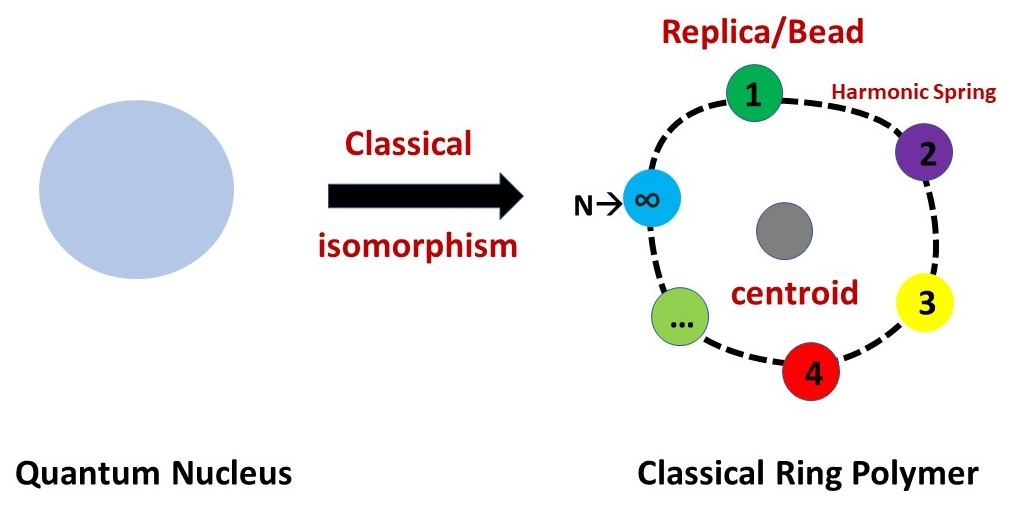
\includegraphics[width=12cm ]{./Comp_methods/Figures/mapping.jpg}
    \caption{The classical isomorphism of a quantum nucleus into a classical ring polymer. The mapping is exact in the limit ${N\to\infty}$.}
    \label{fig:mapping}
\end{figure}


\noindent where the average is over the canonical microstates. An exact description of the quantum  nucleus is only achieved in the limit where the number of beads ($N$) in the ring polymer tends to $\infty$. The interaction among the collection of quantum nuclei is now transformed into an interaction of ring polymers with each bead from one ring polymer interacting with the corresponding beads of other ring polymers. The quantum partition function for the classically isomorphed ring polymers is written below:



\begin{align}
    &Z^{Qt}(\beta)\notag\\
                 &=Tr[e^{-\beta\hat{H}_{nuc,0}(\textbf{P},\textbf{R})}]\label{QPF-7-33}\\ 
                 &=Tr\bigg[\bigg(e^{-\beta_N\hat{H}_{nuc,0}(\textbf{P},\textbf{R})}\bigg)^N\bigg]\label{QPF-7-4}\\
                 &=\lim_{N\to\infty}  \prod_{I=1}^{n_n} (\frac{M_I}{2\pi \hbar^2 \beta_N})^{\frac{3N}{2}} \int_{}^{} \bigg(\prod_{I=1}^{n_n} \prod_{j=1}^{N} d\vec{R}^{j}_{I}\bigg) \quad e^{-\beta_N \sum_{j=1}^{N}    \bigg[\hat{V}^{BO}_{nuc,0}(\textbf{R}^{j})+ \sum_{I=1}^{n_n} \frac{M_I\omega^2}{2}(\vec{R}^{j}_{I}-\vec{R}^{j-1}_{I})^2\bigg]}\label{QPF-7-2}          
\end{align}


\noindent where $n_n$ is the number of nuclei, $M_I$ is the mass of the $I^{th}$ nucleus, $\beta_N=\frac{\beta}{N}$, $\vec{R}^j$ is the position of the $j^{th}$ bead of the ring polymer  and $\omega$ ($= \frac{1}{\beta_N \hbar}$ is the frequency of the harmonic spring between any two beads. The derivation of the quantum partition function (equation \ref{QPF-7-4}) into the partition function of the classical ring polymer (equation \ref{QPF-7-2}) is not mentioned for brevity. However, the derivation includes two prominent quantum mechanical  exploits: (i) the symmetric ``Trotter factorization" of the nuclear Hamiltonian and (ii) the induction of $N-1$ (where $\lim_{N\to\infty}$) position (momenta) eigenstates. The above expression is exact in the limit $N$ tends to $\infty$. However, in order to solve a tractable solution, the value of $N$ needs to be converged. A finite value of $N$ introduces the first approximation to the quantum partition function ($Z_N$) and is given by:

\begin{align}
Z_N&=\prod_{I=1}^{n_n} (\frac{M_I}{2\pi \hbar^2 \beta_N})^{\frac{3N}{2}} \int_{}^{} \bigg(\prod_{I=1}^{n_n} \prod_{j=1}^{N} d\vec{R}^{j}_{I}\bigg) \quad e^{-\beta_N \sum_{j=1}^{N}    \bigg[\hat{V}^{BO}_{nuc,0}(\textbf{R}^{j})+ \sum_{I=1}^{n_n} \frac{M_I\omega^2}{2}(\vec{R}^{j}_{I}-\vec{R}^{j-1}_{I})^2\bigg]}\label{QPF-7-5}
\end{align}
 
 \noindent The classical isomorphism of the quantum nucleus into a classical ring polymer maps the quantum problem into a classical problem of $N$ dimensions. 


\subsubsection*{Imaginary Time Path Integrals}

\noindent A partition function provides the statistical information of the system and is ignorant of the dynamics. However, it is important to understand how the system propagates from one microstate to another. The quantum dynamics of a nuclear system is described by the time dependent nuclear SE with Hamiltonian $\hat{H}_{nuc}$. The evolution of the state of the system from time $t_o$ to $t$ is given by: 

\begin{align}
    \label{QPF-7}
    &i\hbar \frac{\partial}{\partial t}\ket{\Phi(t)}=\hat{H}\ket{\Phi(t)}\\
    &\ket{\Phi(t)} = e^{\frac{-i\hat{H}_{nuc}(t-t_{0})}{\hbar}}\ket{\Phi(t_{0})}=\hat{U}(t)\ket{\Phi(t_{0})}
\end{align}

\noindent where $\hat{U}(t)$ is the quantum time evolution operator. Let us assume, during the time evolution from $t_o$ to $t$, the system moves from $\vec{R}^o$ to $\vec{R}$ such that the state of the system at $\vec{R}$ ($\langle \vec{R} | \Phi(t)\rangle$) is represented as:

\begin{align}
    \label{QPF-8}
      \langle \vec{R} | \Phi(t)\rangle &= \ket{\Phi(\vec{R},t)}\notag\\
      &=\bra{\vec{R}}\hat{U}(t)\ket{\Phi(t_{0})}\notag\\
      &=\int_{}^{}d\vec{R}^o\quad \bra{\vec{R}}\hat{U}(t)\ket{\vec{R}^o}\bra{\vec{R}^o}\ket{\Phi(t_{0})}\notag\\
      &=\int_{}^{}d\vec{R}^o\quad \bra{\vec{R}}\hat{U}(t)\ket{\vec{R}^o}\ket{\Phi(\vec{R}^{o},t_{0})}\notag\\
      &=\int_{}^{}d\vec{R}^o\quad \kappa(\vec{R},\vec{R}^o,t)\ket{\Phi(\vec{R}^{o},t_{0})}
\end{align}

\noindent where $\kappa(\vec{R},\vec{R}^o,t)$ is the ``time evolution amplitude" and forms the heart of the path integral formulation of quantum mechanics. The derivation of $\kappa(R,R^o,t)$ (out of the scope of this thesis) leads to the infinite paths the nuclear system takes to go from ($R^o$ at time $t_o$) to ($R$ at time $t$) which eventually forms the basis of path integrals. The ring polymers can be linked to be the evolution of the path integrals from $R^o$ to $R^o$ in imaginary time  of $\beta\hbar$ time length. The imaginary time propagation is invoked using the Wick rotation of the quantum Boltzmann operator ($e^{-\beta \hat{H}}$). The correlation between the quantum evolution operator ($e^{\frac{-i\hat{H}t}{\hbar}}$) with the Boltzmann operator ($e^{-\beta \hat{H}}$) is shown using the following equivalence:


\begin{align}
    \label{QPF-9}
    \hat{U}(t)=&e^{\frac{-i\hat{H}t}{\hbar}}\equiv e^{-\beta \hat{H}}\notag\\
    &\rightarrow \frac{-i\hat{H}t}{\hbar} =-\beta \hat{H}\notag\\
    &\rightarrow it= \hbar\beta; \quad \beta = it/\hbar
\end{align}

\noindent Hence, the classical isomorphism is also known as the imaginary time path integrals or simply path integrals. 
%------------------------------------------------------------------------------------------------------------------------------------------------------------------------------

\section{Molecular Dynamics (MD) Simulation: Sampling of the BO-PES}
\label{MD}
\noindent The  canonical partition function provides a mathematical representation to the BO-PES at thermal equilibrium. Monte Carlo and Molecular dynamics (MD) are the most common methods to sample any PES. In this thesis, MD is used to sample BO-PES. Depending on the description of the nuclei as quantum or classical, two distinct MD simulations have been used. They are (i) classical nuclei MD, which includes Born-Oppenheimer MD (BOMD) and Quantum Mechanics Molecular Mechanics MD (QMMM MD), and (ii) quantum nuclei MD which includes Path Integral Generalized Langevin Equation based MD\cite{ceriotti2012efficient} (PIGLET). 
%and thermostatted  Ring Polymer MD\cite{rossi2018fine} (t-RPMD). 

\noindent The next subsection very briefly describes the various MD simulation techniques undertaken in this thesis.          
%------------------------------------------------------------------------------------------------------------------------------------------------------------------------------

\subsection{Classical Nuclei MD: Born-Oppenheimer MD (BOMD)}

\subsubsection*{Hamiltonian}

\noindent The nuclear Hamiltonian corresponding to the classical partition function (equation \ref{CPF-1-4}) is  separable and consists of the kinetic ($\hat{T}_{nuc}(\textbf{P})$) and Born-Oppenheimer potential energy ($\hat{V}^{BO}_{nuc,0}(\textbf{R})$) terms. The expression for the classical nuclear Hamiltonian is as follows: 
\begin{align}
    \label{BOMD-1}
    &H^{cl,nuc}=H^{cl}_{kin}+H^{cl}_{pot}\\
    &H^{cl}_{kin}=\hat{T}_{nuc}(\textbf{P}); H^{cl}_{pot}=\hat{V}^{BO}_{nuc,0}(\textbf{R})
\end{align}

\subsubsection*{Propagator}

\noindent The microstates of $Z^{Cl}$ are sampled using a classical propagator. In BOMD simulations, the classical propagation is achieved through the Lagrangian ($\mathcal{L}_{BOMD}$) formulation of classical mechanics, where the Lagrangian ( $\mathcal{L}$) is given by:

\begin{align}
    \label{BOMD-2}
    \mathcal{L}_{BOMD}&=\hat{T}_{nuc}(\textbf{P})-\hat{V}^{BO}_{nuc,0}(\textbf{R})\\ 
                       &=\sum_{I=1}^{n_n}(\frac{M_I\Dot{\Vec{R_I}}^2}{2})-\hat{V}^{BO}_{nuc,0}(\textbf{R})
\end{align}

\noindent $\mathcal{L}_{BOMD}$ is then used in the Euler-Lagrange equation to integrate the equation of motion based on the velocity Verlet scheme.

\begin{align}
    \label{BOMD-3}
    &\frac{d}{dt}\frac{\partial \mathcal{L}_{BOMD}}{\partial \Dot{\Vec{R_I}}} = \frac{\partial \mathcal{L}_{BOMD}}{\partial \Vec{R_I}}\\
%    &\textbf{M}\ddot{\textbf{R}}=\textbf{F}
\end{align}

\noindent The thermostat used to maintain thermal equilibrium in the BOMD simulation is  the ``Canonical Sampling through Velocity Rescaling\cite{bussi2007canonical}" (CSVR). The CSVR thermostat rescales the velocity of all the particles (on the basis of equipartition theorem) so that the temperature of the system remains uniform and constant.  
%------------------------------------------------------------------------------------------------------------------------------------------------------------------------------

\subsection{Classical Nuclei MD : Quantum Mechanics Molecular Mechanics MD (QMMM MD)}

\subsubsection{Hamiltonian}
\noindent As mentioned in section \ref{qmmm-sec} , the system of atoms is divided into two regions (i) the QM  subsystem and (ii) the MM subsystem. Therefore, the nuclear Hamiltonian is modified to incorporate the two subsystems and is given by the following equation:

\begin{align}
    \label{QMMM-MD}
    H_{nuc}^{QMMM}=H^{QM}_{nuc} + H^{MM}_{nuc}
\end{align}

\subsubsection{Propagator}

QMMM MD, alike BOMD, uses the same classical propagator for obtaining the equation of motions. However, the force-mixing scheme of QMMM  uses two sets of forces calculated from the two theories (DFT and FF). Therefore, the Lagrangian for the two subsystem ($\mathcal{L}^{QM}$ and $\mathcal{L}^{MM}$) are different. Moreover, there is dynamic transfer of atoms between the two regions which necessitates the use of a stronger Adaptive Langevin\cite{jones2011adaptive} thermostat. The Adaptive Langevin (Ad-LE) thermostat is a combination of Langevin thermostat  and Nose–Hoover thermostat where the former ensures ergodicity whereas the latter compensates for the loss in energy conservation. The Lagrangian and the equation of motion gets modified in the presence of the Adaptive Langevin thermostat.

\begin{align}
    \label{QMMM-1}
    &\mathcal{L}^{QM}_{Ad-LE}=\mathcal{L}^{QM}+\mathcal{L}_{Ad-LE}\\
    &\mathcal{L}^{MM}_{Ad-LE}=\mathcal{L}^{MM}+\mathcal{L}_{Ad-LE}
\end{align}


%------------------------------------------------------------------------------------------------------------------------------------------------------------------------------


\subsection{Quantum Nuclei MD: Path Integral Generalized Langevin Equation Thermostat (PIGLET)}

\subsubsection{Hamiltonian}

The expression for the canonical partition function for $N$ bead ring polymer ($Z_N$) integrates out the momenta of the nuclei. This form of partition function is sampled using Monte Carlo. However, in order to have a MD simulation, the momenta of the nuclei needs to be re-introduced into $Z_{N}$. The re-introduction of momenta becomes a tool for MD and can be tuned for effective  sampling. The tuning is done by changing the physical mass of the nucleus ($M_I$) with a fictitious one ($\tilde{M_I}$). The equation for $Z_N$ due to the reintroduction of the fictitious momenta is given by:


\begin{align}
    \label{QNMD-1}
    Z_{N}&=\prod_{I=1}^{n_n} (\frac{M_I}{2\pi \hbar^2 \beta_N})^{\frac{3N}{2}} \int_{}^{} \bigg(\prod_{I=1}^{n_n} \prod_{j=1}^{N} d\vec{R}^{j}_{I}\bigg) \quad e^{-\beta_N \sum_{j=1}^{N}    \bigg[\hat{V}^{BO}_{nuc,0}(\textbf{R}^{j})+ \sum_{I=1}^{n_n} \frac{M_I\omega^2}{2}(\vec{R}^{j}_{I}-\vec{R}^{j-1}_{I})^2\bigg]}\notag\\ 
    &=\frac{1}{(2\pi\hbar)^{3n_nN}} \bigg(\frac{\textbf{M}}{\Tilde{\textbf{M}}}\bigg)^{\frac{3N}{2}} \int_{}^{} \bigg(\prod_{I=1}^{n_n} \prod_{j=1}^{N} d\vec{R}^{j}_{I}\bigg) \bigg(\prod_{I=1}^{n_n} \prod_{j=1}^{N} d\vec{P}^{j}_{I}\bigg)\notag\\ 
    & \quad e^{-\beta_N \sum_{j=1}^{N}  \bigg[\hat{V}^{BO}_{nuc,0}(\textbf{R}^{j})+ \sum_{I=1}^{n_n} \frac{M_I\omega^2}{2}(\vec{R}^{j}_{I}-\vec{R}^{j-1}_{I})^2 + \sum_{I=1}^{n_n} \frac{(\vec{P_I}^j)^2}{2\Tilde{M}}\bigg]}\notag\\     
\end{align}

%%%%%%%%%%%%%%%%%%%%%%%%%%%%%%%%%%%%%%%%%%%%%%%%%%%%%%%%%%%%%%%ERROR
   


 \noindent The corresponding Hamiltonian is known as the ``PIMD" Hamiltonian ($\hat{H}^{pimd}_{N,nuc,0}(\textbf{P}^{(j)},\textbf{R}^{(j)})$) where $\textbf{P}^{(j)}$ and $\textbf{R}^{(j)}$ are the set of momenta and position vectors for all beads and nuclei. $\Tilde{\textbf{M}}$ and $\textbf{{M}}$ are the fictitious and physical/real mass matrices of all the nuclei. The associated MD is known as the ``Path Integral Molecular Dynamics (PIMD)". The expression for PIMD Hamiltonian is given below:

\begin{align}
\label{QNMD-2}
    \hat{H}^{pimd}_{N,nuc,0}(\textbf{P}^{(j)},\textbf{R}^{(j)})=\sum_{j=1}^{N}  \bigg[\hat{V}^{BO}_{nuc,0}(\textbf{R}^{j})+ \sum_{I=1}^{n_n} \frac{M_I\omega^2}{2}(\vec{R}^{j}_{I}-\vec{R}^{j-1}_{I})^2 + \sum_{I=1}^{n_n} \frac{(\vec{P_I}^j)^2}{2\Tilde{M_I}}\bigg]
\end{align}

\noindent  However, restricting the choice of the fictitious momenta to the actual momenta of the nuclei constructs the ``RPMD" Hamiltonian ($\hat{H}^{rpmd}_{N,nuc,0}(\textbf{P}^{(j)},\textbf{R}^{(j)})$) and the subsequent ``Ring Polymer Molecular Dynamics (RPMD)". The expression for RPMD hamiltonian is given below: 

\begin{align}
\label{QNMD-3}
    \hat{H}^{rpmd}_{N,nuc,0}(\textbf{P}^{(j)},\textbf{R}^{(j)})=\sum_{j=1}^{N}  \bigg[\hat{V}^{BO}_{nuc,0}(\textbf{R}^{j})+ \sum_{I=1}^{n_n} \frac{M_I\omega^2}{2}(\vec{R}^{j}_{I}-\vec{R}^{j-1}_{I})^2 + \sum_{I=1}^{n_n} \frac{(\vec{P_I}^j)^2}{2M_I}\bigg]
\end{align}

\noindent The terms RPMD and PIMD are used interchangeably in this thesis as both refer to the RPMD Hamiltonian where the real masses of the nuclei are used.

\subsubsection{Propagator}

\noindent In PIMD or RPMD, the microstates of $Z_N$ are also sampled using the classical dynamics of the nuclei. The classical propagation is based on the classical Liouvillian formulation of the Hamiltonian equation of motion. The Hamiltonian equations of motion are as follows: 

\begin{align}
    \label{QNMD-4}
    &\frac{d\textbf{R}^{(j)}}{dt}=\frac{\partial\hat{H}^{rpmd}_{N,nuc,0}(\textbf{P}^{(j)},\textbf{R}^{(j)})}{\partial \textbf{P}^{(j)}}\notag\\
    &\frac{d\textbf{P}^{(j)}}{dt}=-\frac{\partial\hat{H}^{rpmd}_{N,nuc,0}(\textbf{P}^{(j)},\textbf{R}^{(j)})}{\partial \textbf{R}^{(j)}}\notag\\
\end{align}

\noindent The classical Liouvillian propagator ($e^{iLt}$) and its corresponding equations of motion are as follows:

\begin{align}
    \label{QNMD-5}
    &iL=\bigg(\frac{\partial\hat{H}^{rpmd}_{N,nuc,0}(\textbf{P}^{(j)},\textbf{R}^{(j)})}{\partial \textbf{P}^{(j)}}\bigg) \frac{\partial}{\partial \textbf{R}^{(j)}} + \bigg(-\frac{\partial\hat{H}^{rpmd}_{N,nuc,0}(\textbf{P}^{(j)},\textbf{R}^{(j)})}{\partial \textbf{R}^{(j)}}\bigg) \frac{\partial}{\partial \textbf{P}^{(j)}}
\end{align}

\begin{align}
    \label{QNMD-55}
    &\textbf{R}^{(j)}(t)=e^{iLt}\textbf{R}^{(j)}(t_o)\notag\\
    &\textbf{P}^{(j)}(t)=e^{iLt}\textbf{P}^{(j)}(t_o)
\end{align}

\noindent The classical evolution of interacting ring polymers (Eq. \ref{QNMD-55}) is difficult to integrate and is often done in an unexact fashion. Therefore, a more practical way is to split the Hamiltonian into two parts namely (i) Hamiltonian for the free ring polymer ($\hat{H}^{frp}_{N,nuc,0}$) and (ii) Hamiltonian for the potential between the ring polymers ($\hat{H}^{pot}_{N,nuc,0}$) and evolve the individual split up Hamiltonians exactly. Here and after, the dependence of the RPMD Hamiltonian on the position and momenta vectors is dropped for simplicity. The readjusted expression for the complete Hamiltonian is as follows:

\begin{align}
\label{QNMD-6}
    \hat{H}^{rpmd}_{N,nuc,0}&=\hat{H}^{pot}_{N,nuc,0}+\hat{H}^{frp}_{N,nuc,0}\\
                             &=\sum_{j=1}^{N}  \bigg[\hat{V}^{BO}_{nuc,0}(\textbf{R}^{j})\bigg] + \sum_{j=1}^{N} \sum_{I=1}^{n_n} \bigg[\frac{M_I\omega^2}{2}(\vec{R}^{j}_{I}-\vec{R}^{j-1}_{I})^2 + \frac{(\vec{P_I}^j)^2}{2M_I}\bigg]
\end{align}

\noindent Each part of the Hamiltonian is associated with their respective classical propagators obtained approximately by the symmetric Trotter factorization of the complete classical propagator. The resultant equation for the split up classical propagator for a $\Delta t$ time step is as follows:

\begin{align}
\label{QNMD-66}
    &e^{iL\Delta t}\simeq e^{iL_{pot}\frac{\Delta t}{2}}e^{iL_{frp}\Delta t}e^{iL_{pot}\frac{\Delta t}{2}}
\end{align}

\noindent where $e^{iL_{frp}}$ is associated with $\hat{H}^{frp}_{N,nuc,0}$ and $e^{iL_{pot}}$ is associated with $\hat{H}^{pot}_{N,nuc,0}$. The overall algorithm\cite{ceriotti2010efficient} for integrating the equations of motion for a $\Delta t$ is as follows (dropping the vector sign over $\vec{P}$ and $\vec{R}$ for simplicity):

\begin{align}
    &P_I^{j} \leftarrow P_I^{j} - \frac{\Delta t}{2}\frac{\partial V(\textbf{R}^j)}{\partial R_I^j}\label{QNMD-71}\\
    &\Tilde{P_I^{k}} \leftarrow \sum_{j=1}^{N}P_I^{j}C_{jk};\quad \Tilde{R_I^{k}} \leftarrow \sum_{j=1}^{N}R_I^{j}C_{jk} \label{QNMD-72}\\
    &\begin{bmatrix}
        \Tilde{P_I^{k}} \\ \Tilde{R_I^{k}} 
    \end{bmatrix}
    \leftarrow\begin{bmatrix}
        cos (\omega_{k}\Delta t) \quad \quad -M_I \omega_{k} sin (\omega_{k}\Delta t) \\
        \frac{1}{M_I\omega_{k}}sin (\omega_{k}\Delta t) \quad \quad cos (\omega_{k}\Delta t)
    \end{bmatrix}
    \begin{bmatrix}
        \Tilde{P_I^{k}} \\ \Tilde{R_I^{k}} 
    \end{bmatrix}\label{QNMD-73}\\
        &P_I^{k} \leftarrow \sum_{k=0}^{N-1}C_{jk}\Tilde{P_I^{j}};\quad R_I^{k} \leftarrow \sum_{k=0}^{N-1}C_{jk}\Tilde{R_I^{j}} \label{QNMD-74}\\
    &P_I^{j} \leftarrow P_I^{j} - \frac{\Delta t}{2}\frac{\partial V(\textbf{R}^j)}{\partial R_{I}^{j}}\label{QNMD-75}
\end{align}

\noindent The first step (Eq. \ref{QNMD-71}) is the exact propagation of the ring polymer momenta by $\Delta t/2$ time step under the influence of $\hat{H}^{pot}_{N,nuc,0}$. The second step (Eq. \ref{QNMD-72}) is the transformation of the cartesian representation of the ring polymer to the normal mode representation where $C_{jk}$ is the orthogonal transformation matrix for an even N.

\begin{align}
    C_{jk}=
    \begin{cases}
    \sqrt{1/N}, &k=0\\
    \sqrt{2/N}cos(2\pi jk/N),&1\leq k \leq N/2-1\\
    \sqrt{1/N}(-1)^j, &k=N/2\\
    \sqrt{2/N}sin(2\pi jk/N),&N/2+1\leq k \leq N-1
    \end{cases}
\end{align}


\noindent The third equation (Eq. \ref{QNMD-73}) is an exact evolution of the ring polymer through a time step of $\Delta t$ in the normal mode representation under the influence of $\hat{H}^{frp}_{N,nuc,0}$. The normal mode frequency of the ring polymer is given as follows:
\begin{equation}
 \omega_k= 2\omega sin(k\pi/N)   
\end{equation}

\noindent The fourth and fifth steps (Eq. \ref{QNMD-74} and Eq. \ref{QNMD-75}) are the transformation of the ring polymer from the normal mode to cartesian representation and the further propagation of the evolved (cartesian) ring polymer by a $\Delta t/2$ time step under the influence of $\hat{H}^{pot}_{N,nuc,0}$ respectively.

\noindent As mentioned earlier, the quantum partition function is exact in the limit where the number of beads of the ring polymer approaches $\infty$. However, an upper cap on the number of beads is obtained using convergence tests. This converged number of beads is proportional to the maximum frequency of the inter nuclear vibration of the physical system and inversely proportional to the temperature ($N \propto \frac{\omega_{max}}{T}$). As a result, at low temperatures and/or high physical vibration, the number of beads needed for converging physical properties becomes large. An efficient way to accelerate the convergence with respect to the number of beads is to couple the RPMD dynamics with a non-equilibrium coloured noise Langevin dynamics\cite{ceriotti2010novel,ceriotti2010efficient,ceriotti2012efficient} that introduces frequency dependent quantum fluctuations to mimic the zero point energy of the system consisting of multi-dimensional harmonic oscillators which also applies to anharmonic systems\cite{ceriotti2011accelerating}. This state of the art thermostatting technique by a non-equilibrium Generalized Langevin equation based thermostat (GLET) of the RPMD simulation is known as Path Integral Generalized Langevin Equation Thermostat\cite{ceriotti2012efficient} (PIGLET). The coupling of the GLET dynamics with the RPMD dynamics modifies the Liouvillian (Eq. \ref{QNMD-66}) in the following manner:  

\begin{align}
\label{QNMD-666}
    &e^{iL\Delta t}\simeq  e^{iL_{GLET}\frac{\Delta t}{2}} e^{iL_{pot}\frac{\Delta t}{2}}e^{iL_{frp}\Delta t}e^{iL_{pot}\frac{\Delta t}{2}} e^{iL_{GLET}\frac{\Delta t}{2}}
\end{align}

\noindent This results in introducing thermostat dynamics twice per step, immediately before and immediately after the RPMD dynamics (Eq. \ref{QNMD-71}-\ref{QNMD-75}). A very brief description regarding the stochastic dynamics is presented below. 

\subsubsection{Generalized Langevin Equation based Thermostat: Stochastic dynamics}

Thermostats are used as temperature control to sample the canonical distribution of positions and momenta of atoms in classical (Newtonian) dynamics. Since ring polymers make the system stiff, Noose-Hoover chain thermostat\cite{martyna1992nose,tuckerman1993efficient} is generally used with RPMD dynamics to obtain ergodicity and is considered a gold standard for perofming path integral molecular dynamics. The Noose-Hoover chain dynamics is detrministic and is applied immediately before and immediately after the RPMD dynamics and is reported elsewhere\cite{ceriotti2010efficient}. Alternatively, Ceriotti and Parinello\cite{ceriotti2010efficient} showed a simple stochastic (white/Markovian) Langevin thermostat, primarily used to model brownian motion, can also be used with path integral simulation (PILE) to ensure ergodicity. The equations of motion for the Langevin dynamics are given below, which similar to Noose-Hoover chain are applied immediately before and after the RPMD dynamics (Eq. \ref{QNMD-71}-\ref{QNMD-75}). 

\begin{align}
    \label{QNMD-91}
     &\Tilde{P_I^{k}} \leftarrow \sum_{j=1}^{N}P_I^{j}C_{jk}\notag\\
      &\Tilde{P_I^{k}} \leftarrow c_1^{k}\Tilde{P_I^{k}} + \sqrt{\frac{M_I}{\beta_N}}c_2^{k}\xi_I^{k}\notag\\ 
      &{P_I}^{j} \leftarrow \sum_{k=0}^{n-1} C_{jk} \Tilde{P_I^{k}}
\end{align}

\noindent where $\xi_I^{k}$ is an independent Gaussian number (random noise term). The coefficients $c_1^{k}$ and $c_2^{k}$ can be written as as follows:

\begin{equation}
    c_1^{k}=e^{(-\Delta t/2)\gamma^{k}} ; \quad  c_2^{k}=\sqrt{1-[c_1^{k}]^2}\label{QNMD-92}\\    
\end{equation}

\noindent where $\gamma^{k}$ is the normal mode friction coefficients. In the view of optimal sampling of the free (non-interacting) ring polymers, $\gamma^{k}$ is given as follows:

\begin{align}
    \label{QNMD-922}
    &\gamma^{k}=
    \begin{cases}
    \sqrt{1/\tau_{0}}, &k=0\\
    2\omega_{k}, &k > 0\\
    \end{cases}    
\end{align}

 \noindent In this approach, the ring polymer normal mode is separated into the centroid ($k=0$) mode with an autocorrelation time of $\tau_0$ and excited modes ($k > 0$) with an autocorrelation time constant of  $2\omega_k$ where $\omega_k$ is the ring polymer frequency of the excited modes. 

 \noindent However, Ceriotti and coworkers showed that a coloured noise (non-Markovian with a memory kernel) Generalized Langevin Thermostat\cite{ceriotti2009langevin} instead of the simple Langevin thermostat gives more control over the static and dynamical properties. This was achieved by converting the non-Markovian (memory) dynamics into a Markovian one\cite{ceriotti2010novel} by extending the phase space with additional momenta bilinearly coupled to the physical momentum. This control over the dynamics prompted Ceriotti and coworkers\cite{ceriotti2009nuclear} to  include quantum corrections to the classical dynamics. They fit the correlation function of the random noise to match the quantum fluctuations in position and momenta of the various vibrational modes of the system in such a way that minimal apriori knowledge about the system is required. As a result of this fitting procedure, the preservation of equivalence between the friction and noise terms, as dictated by the fluctuation-dissipation theorem, is compromised, leading to the emergence of non-equilibrium dynamics. The equation of quantum fluctuations for the position and momentum has the following form.

  \begin{equation}
    c_{RR}(\omega) = \frac{1}{\omega^2} c_{PP}(\omega) = \frac{\hbar}{2\omega} coth \frac{\hbar \omega}{2k_BT} \label{QNMD-97}    
\end{equation}


\noindent where $\omega$ is the frequency of the normal mode, $c_{RR}$ and $c_{PP}$ are the quantum mechanical thermal expectation value of the squared position ($R^2$) and momenta ($P^2$) respectively. This quantum thermostat (QT) was coupled to path integral methods\cite{ceriotti2011accelerating} in order to compliment the remainder quantum fluctuations incorporated using the ring polymer. The corresponding equation of motion is analytically solvable if the physical vibrations in the system are within the harmonic limit but are successfully extended to strongly anharmonic systems\cite{ceriotti2011accelerating} through numerical solutions. The corresponding equations of motions for the PI $+$ GLE method before and after the RPMD dynamics are as follows: 
%\begin{equation}
%    \frac{1}{P} \sum_{k=0}^{N-1}c_{RR}(\omega) = \frac{\hbar}{2\omega} coth \frac{\hbar \omega}{2k_BT} \label{QNMD-98}
%\end{equation}

\begin{equation}
\mathbf{P_{I}^{j}} \leftarrow \mathbf{C_1} \mathbf{P_{I}^{j}} + \sqrt{\frac{M_I}{\beta_{N}}} \mathbf{C_{2}} \boldsymbol{\xi_{I}^{j}} \notag
\end{equation}


\begin{equation}
    \textbf{P}_I^{j} = 
    \begin{bmatrix}
        P_I^{j} \\ \textbf{s}_I^{j}
    \end{bmatrix} \label{QNMD-95}
\end{equation}

\noindent where $\textbf{P}_I^{j}$ is the column vector containing the momentum of the $I^{th}$ nuclei for the $j^{th}$ bead and its additional momenta ($\textbf{s}_I^{j}$;\quad $s_{I,1}^j$ , $s_{I,2}^j$ , ...,$s_{I,n_s}^j$) for enforcing Markovian dynamics in extended phase phase. $\boldsymbol{\xi_{I}^{j}}$ is a vector of $n_s + 1$ independent Gaussian numbers. The $\textbf{C}_1$ and $\textbf{C}_2$ are matrices related to the friction and noise terms respectively and are fitted to enforce quantum fluctuations in the position and momenta. They depend on the number of beads, the additional momenta needed to extend the phase space, the temperature and the highest physical frequency of the system along with the range of frequency in which the quantum corrections are to be applied. The expression and details regarding the matrices, the equations of motion and the fitting procedure can be found in the thesis\cite{ceriotti2010novel} and related publications\cite{ceriotti2012efficient,ceriotti2011accelerating} by Michele Ceriotti (\underline{https://www.epfl.ch/labs/cosmo/}).


%\begin{equation}
%    \textbf{C}_1 = e^{(-\Delta t/2)\gamma^{T}}; \quad \textbf{C}_2^{T}\textbf{C}_2 = I- \textbf{C}_1^{T}\textbf{C}_1 \label{QNMD-94}
%\end{equation}

%\begin{equation}
%    \textbf{P}_I^{j} \leftarrow \frac{-\partial V(\textbf{R}^j)}{\partial R_I^j} + \textbf{C}_1\textbf{P}_I^{j} + \sqrt{\frac{M_I}{\beta_N}}\textbf{C}_2\textbf{\xi}_I^{j} \label{QNMD-96}
%\end{equation}

\noindent Further, it was observed that the PI $+$ GLE method consists of the quantum kinetic energy which is dependent on the centroid mode of the ring polymer leading to bead-bead correlations which slows down its convergence with respect to the number of beads. The solution to this problem was addressed by Ceriotti and coworkers\cite{ceriotti2012efficient} by coupling a classical (equilibrium) thermostat to the centroid mode of the ring polymer and applying to each other normal mode of the ring polymer with the non-equilibrium frequency dependent GLE thermostat. This method ensures the fast convergence of both the potential and quantum kinetic energy with respect to the number of beads and is the ``\textbf{PIGELT}" method used in this thesis. The $\textbf{C}_1$ and $\textbf{C}_2$ matrices obtained through the fitting procedure is freely available at \underline{http://gle4md.org/}. This PIGLET method with respect to PIMD has been successful in reducing the number of beads by a factor 4 and more\cite{ceriotti2010efficient} for structural properties. For water at 300 K, the structural properties are converged over 6 beads of PIGLET compared to the 32 beads for PIMD\cite{ceriotti2012efficient}. Other noticeable example is the structural description of the Zundel cation at low temperatures is strongly benefitted from the use of PIGLET simulation\cite{schran2018converged}. The authors also compare PIGLET with another variant of quantum thermostatting with PIMD named Path Integral Quantum Thermal Bath (PIQTB\cite{schran2018converged,brieuc2016quantum}). 



